\chapter{An Augmented Quantum Threshold Scheme}
\label{ch3}

As we have shown above, one of the main limitations of QC comes from the no-cloning theorem. The first idea we pose attempts to circumvent this limitation. 

If we begin with two identical copies of a quantum state, then what does this do, if anything, to change the limitations surrounding the value of $t$ with respect to $n$? What if we have $k$ copies? What schemes are realizable in this new formulation? In this section, we will explore the properties of such a scheme. We will call this an augmented quantum threshold scheme. Let us formalize this idea and explore its consequences below:

\theoremstyle{definition}
\begin{definition}{Augmented Quantum Threshold Scheme.}
    \label{defn:augmented-qts}
     This is a QTS that assumes that we being with $k$ identical copies of a quantum state prepared in advance. As with the normal QTS, we need at least $t$ individuals to come together to recover the secret quantum state. We will denote an augmented QTS as $((t,n,k))$.
\end{definition}

\section{Preliminary thoughts}

Let's consider the case of $k=2$. If we consider just the consequences of the no-cloning theorem, an extension of \thmref{thm:qss-disjoint} can be posed as follows:

\begin{theorem}
    \label{thm:three-authorized}
    In any valid $((t,n,2))$ scheme, any three authorized subsets cannot be pair-wise disjoint.
\end{theorem}

And a generalization to the case with $k$ identical copies:

\begin{theorem}
    \label{thm:k-authorized}
    In any valid $((t,n,k))$ scheme, any $k+1$ authorized subsets cannot be pair-wise disjoint.
\end{theorem}

We can also extend \thmref{thm:qts} in a similar manner:

\begin{theorem}
	\label{thm:qts2}
	A QTS $((t,n, 2))$ exists only if $t > \frac{n}{3}$.
\end{theorem}

\begin{theorem}
	\label{thm:qtsk}
	A QTS $((t,n, k))$ exists only if $t > \frac{n}{k+1}$.
\end{theorem}

Each of the proofs of these theorems are almost identical to that of \thmref{thm:qss-disjoint}. However, these theorems only present to us what schemes are not immediately ruled out by the no-cloning theorem. Figuring out methods of realizing these schemes is a different question. It is not immediately obvious that Gottesman's \thmref{thm:monotone-gamma} applies to augmented threshold schemes.

\section{A Union of Access Structures Approach}

The simplest case that is non-trivial is to consider a $((2,4,2))$ scheme. Using 2 identical copies of a quantum state, is it possible to implement a scheme among 4 individuals such that only 2 or more people need to come together to recover the secret? The answer is yes.

The strategy that we will use will employ a strategy where we take the union of two valid access structures, each using only one quantum state each. Let the two copies of our quantum secret be $\ket{\psi_1}, \ket{\psi_2}$, and let the participants be labeled $p_1, p_2, p_3, p_4$. \fref{fig:2-4-2} shows how we implement the scheme. Each node corresponds to one participant, and the blue edges denote authorized subsets of size 2 that are a part of the access structure $\Gamma_1$ of $\ket{\psi_1}$. Red edges correspond to $\Gamma_2$, which is the access structure of $\ket{\psi_2}$.


\begin{figure}[ht]
	\begin{center}
        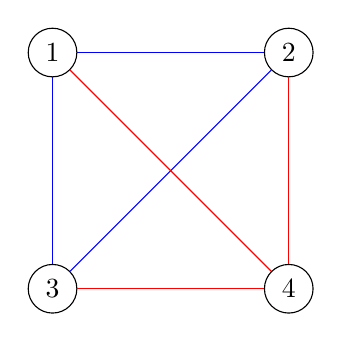
\begin{tikzpicture}[scale=3,auto=left,every node/.style={circle,draw,fill=white}]
          \node (n1) at (0,1) {1};
          \node (n2) at (1,1) {2};
          \node (n3) at (0,0) {3};
          \node (n4) at (1,0) {4};
          
          \draw [blue] (n1) -- (n2);
          \draw [blue] (n3) -- (n2);
          \draw [blue] (n1) -- (n3);
          \draw [red] (n1) -- (n4);
          \draw [red] (n2) -- (n4);
          \draw [red] (n3) -- (n4);
        \end{tikzpicture}
	\end{center}
	\caption{An image of the access structure for a $((2,4,2))$ threshold scheme, using two copies of the quantum secret.}
	\label{fig:2-4-2}
\end{figure}


The scheme is as follows: $\Gamma_1 = \{p_1p_2,p_2p_3,p_3p_1\}$ and $\Gamma_2 = \{p_1p_4,p_2p_4,p_3p_4\}$. Observe that each access structure satisfies \thmref{thm:qss-disjoint}. By \thmref{thm:monotone-gamma}, a $((2,4,2))$ scheme exists.

\subsection{A Better Graphical Representation}

How can we generalize this strategy? Notice that in the case of the $((2,4,2))$ scheme, we need the union $\Gamma_1 \cup \Gamma_2$ to consist of all subsets of size 2. Each of these access structures must satisfy Theorem \ref{thm:qss-disjoint}. So, in general, a $((t,n,k))$ scheme is realizable if we can take all subsets of size $t$ of the $n$ participants and divide them into $k$ groups, where each group consists of an access structure that satisfies Theorem \ref{thm:qss-disjoint}. 

Let's dive deeper into augmented threshold schemes of the form: $((t,n,2))$. What would be useful for us is a representation of this problem that allows us to better reason about the authorized subsets contained in the access structures. The formulation we use in \fref{fig:2-4-2} is a natural one: where each node represents a participant, and the edges represent authorized subsets. However, we run into the problem where we can only properly represent authorized subsets of size 2.

So, instead of representing the participants as vertices and the authorized subsets as edges, we take inspiration from Singh and Srikanth's \cite{singh_assisted_2004} AS graph representation, which we defined in \defref{defn:access-structure-graph}. We \textbf{make each authorized subset a vertex}, and have the edges denote some relationship between the authorized sets. However, we make one modification from their representation. Instead of having an edge between any two authorized sets that overlap, we place an edge between them if they \textbf{do not overlap}. In other words, this is the \textit{complement} of the AS graph.

\begin{definition}{Access Structure Graph Complement.}
    \label{defn:access-structure-graph-complement}
	We define an \textbf{access structure graph} of $\Gamma$ to be the graph $G = (V,E)$, where there is a vertex $v \in V$ for each authorized subset $A \in \Gamma$. The edgeset $E$ contains an edge between each pair of vertices if their corresponding authorized subsets are disjoint.
\end{definition}

The access structure graph complement for \fref{fig:2-4-2} is shown in \fref{fig:2-4-2-graph}. Later in this section, we will explore why using the complement of the AS graph can be beneficial to us:

\begin{figure}[H]
    \centering
	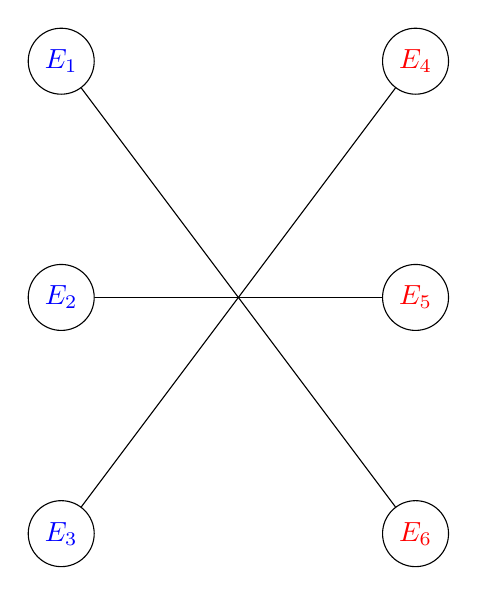
\begin{tikzpicture}[scale=3,every
	node/.style={circle,fill=white}]
      \node [draw,text=blue] (n1) at (0,3)   {$E_1$};
      \node [draw,text=blue] (n2) at (0,2)   {$E_2$};
      \node [draw,text=blue] (n3) at (0,1)   {$E_3$};
      \node [draw,text=red] (n4) at (1.5,3) {$E_4$};
      \node [draw,text=red] (n5) at (1.5,2) {$E_5$};
      \node [draw,text=red] (n6) at (1.5,1) {$E_6$};
      
      \draw [black] (n1) -- (n6);
      \draw [black] (n3) -- (n4);
      \draw [black] (n2) -- (n5);
    \end{tikzpicture}
	\caption{The access structure graph representation for a $((2,4,2))$ scheme.}
    \label{fig:2-4-2-graph}
\end{figure}

The representation illustrated in \fref{fig:2-4-2-graph} is useful to us because properties of the graph now reveal properties of the realizability of their corresponding quantum threshold schemes. Let's bring in the idea of graph coloring introduced in \defref{defn:colors}.

\begin{theorem}
    \label{thm:2-color-access}
    The chromatic color of the access structure graph of $\Gamma$ is 2 if and only if a $((t,n,2))$-threshold quantum secret sharing scheme is valid.
\end{theorem}

This is true because it implies that there does not exist 3 or more authorized subsets that are pairwise-disjoint.

What is even better for $((t,n,2))$ schemes is the fact that another name for graphs with $\chi(G)=2$ is \textbf{bipartite}, which we introduce in \defref{defn:bipartite}.

A quick look at \fref{fig:2-4-2-graph} reveals that the graph is indeed bipartite, again verifying that $((2,4,2))$ is a valid scheme. A well-known result in graph theory is stated below:

\begin{theorem}
	\label{thm:bipartite}
	A graph $G$ is bipartite if and only if $G$ does not contain any odd cycles.
\end{theorem}

We can use \thmref{thm:bipartite} to also show that $((3,6,2))$ is also a valid scheme, but that $((2,5,2))$ and $((3,7,2))$ are \textbf{not} valid schemes. 

For the $((3,6,2))$ scheme, we can take a similar approach to the $((2,4,2))$ scheme and illustrate the access structure graph.

For the $((2,5,2))$ scheme, rather than try to draw an access structure, we find an odd cycle in the access structure graph by listing an ordering of vertices that have edges connecting them: $(1,2), (3,4), (5,1), (2,3), (4,5), (1,2)$. Each integer represents an individual, and each pairing of integers represents an size-2 subset. We find that this path with 5 edges is a cycle, so there is an odd-cycle. Therefore, the graph is not bipartite, so $((2,5,2))$ does not represent a valid augmented quantum threshold scheme. We take a similar approach for $((3,7,2))$, and come to the same conclusion.

In this next section, we seek out more generalized approaches to determining whether or not a scheme is realizable, rather than just illustrating the access structure graph or manually finding odd cycles.

\subsection{Generalization of $((t,n,2))$ Schemes}

Let's continue to consider schemes of the form $((t,n,2))$. Using a similar graphical approach, we will show two results: that all schemes of the form $((t,2t,2))$ are possible, and all schemes of the form $((t, 2t+1, 2))$ are not possible. Thus, the best that we can do with two copies of a share is $((t,2t,2))$. 

% we can realize t,2t schemes
\begin{theorem}
    \label{thm:t-2t-2}
    Quantum threshold schemes of the form $((t,2t,2))$ are realizable using our union of access structures strategy.
\end{theorem}

\begin{proof}
    We will show that there cannot be any odd cycles in the access structure graph representations of these schemes. And then, by \thmref{thm:bipartite}, the graph must be bipartite, and therefore two-colorable. This means that the scheme is realizable. Consider one of the authorized sets, and without loss of generality, let this set have the participants: $\{p_1,\dots,p_t\}$. Then, there is only one possible authorized set that is disjoint from this one: $\{p_{t+1},\dots,p_{2t}\}$. Note that this is true for every single authorized set (of size $t$). Therefore, each vertex has degree exactly equal to 1. We can immediately see that such a graph must be bipartite.
\end{proof}

% we cannot realize t,2t+1 schemes
\begin{theorem}
    \label{thm:t-2t+1-2}
    Quantum threshold schemes of the form $((t,2t+1,2))$ are not realizable using our union of multiple access structures strategy.
\end{theorem}
 
 % the proof is in the pudding 
\begin{proof}
    Let's say we have a set of participants $\mathcal{P} = \{p_1,p_2,\dots,p_{2t+1}\}$. We will denote each authorized subset as an un-ordered set of participants. We will show that the access structure graph representation of these schemes must include an odd cycle. What we are looking for, then, is an ordered list of authorized subsets, $A_1, A_2, \dots, A_r$, such that $A_1=A_r$ and $A_i \cap A_{i+1} = \emptyset \: \forall i \in \{1,\dots,r-1\}$. If $r$ is even, then we have an odd cycle. WTLOG, let's denote the first authorized subset as $\{p_1,\dots,p_{t}\}$. From this set, we can generate a cycle of authorized sets by counting in groups of $t$ modulo $2t+1$. Let's list a series of a few of these sets:
    
    \begin{align*}
        &\{p_1,\dots,p_{t}\} \\ 
        &\{p_{t+1},\dots,p_{2t}\} \\ 
        &\{p_{2t+1},\dots,p_{t-1}\} \\ 
        &\{p_{t},\dots,p_{2t-1}\} \\
        & \vdots \\
        &\{p_{t+3},\dots,p_{1}\} \\ 
        &\{p_{2},\dots,p_{t+1}\} \\ 
        &\{p_{t+2},\dots,p_{2t+1}\} \\ 
        &\{p_1,\dots,p_{t}\} \\ 
    \end{align*}
    
    How many edges are in this cycle? Observe that $t$ and $2t+1$ are relatively, prime, for $t > 2$. This means that there are $2t+1$ edges in this cycle, so we have an odd cycle. For the case that $t=1$, we the result is trivial, because we would have three pair-wise disjoint authorized sets.
\end{proof}






